\chapter{Results}
\label{cha:results}
% This chapter should display the results of your experiments. It should be entirely
% factual, so leave the discussion you draw from it for the Discussion chapter.
%
% You may choose to structure your thesis slightly differently, but the overall 
% approach should be the same.
%
% 1. By now you should have already described your methodology and  evaluation 
%    procedures. There is no reason to discuss these in the results.
% 2. Do not include raw data in the results chapter, leave it for the appendix 
%    or simply don't include it. If you don't think people will refer to it it's
%    probably not worth including.
% 3. Display your results in an informative way. Charts, tables, summaries, etc.
%
% If your results form a complete chapter you can use the conclusion section to
% state how the results answer your hypothesis. If you don't have a spearate
% conclusion chapter make sure you answer the hypothesis as you go. The reader
% should have answers to these before the Discussion.

The problem at hand along with the methodology employed to produce the solution are now well defined. Paired with an understanding of important previous works in this area and the technologies available, the design of each of the components may be given consideration. This chapter will present the designs of the required additions to the Gene-Plex Extractor, as were defined in Section \ref{sec:intro_scope}, Scope. This will include relevant results from stages of the design process, the conducted simulations along with validations and verifications via experimental methods. Through the sections below, the reader will be familiar with the design of each of the components along with the resulting performance of the realised and implemented component.\\

\section{Processor Module}

\subsection{Hardware}

\subsubsection{Thermal Isolation}

The first consideration given to the design of the physical Processor Module was the thermal isolation of the heated and non-heated volumes. While there is no requirement stipulating that only tubes 2 and 3 may be heated, it was deemed  thermally inefficient to heat the entire module. Such a design would also decrease the performance of the controller due to the larger mass to be heated. Therefore, the module was split into two regions, refereed to as the Thermal Region and the Carrier. While the method of isolation needed to be effective to create a stable and controllable thermal system, a number of other design considerations were present:
\begin{enumerate}
	\item[Manufacturability] The design of the thermal isolation method needed to consider the available manufacturing methods and their capabilities. For example, concept A shown in Figure \ref{fig:splitconcepts}, utilized a simple "trench" to create an air gap between the heated and non-heated regions of a single block of aluminium. While this concept satisfied the serviceability and cost objectives, there were a number of physical constraints preventing it from being feasible. Due to the geometry of the cassettes, the trench width was limited to 3mm across. At this size, the maximum depth at which the tooling could cut was stated to be 30mm \cite{Sorenson}. At this depth, not only would a large area of material still connect the two regions, but the cost of machining would be high.
	\item[Serviceability] When considering the serviceability of the product, two main aspects were key. This includes the initial assembly of the device after manufacture along with the periodic maintenance during its operating life. The resulting design must ensure manual assembly is practical and that the replacement of components, such as sensors or heating hardware is considered. 
	\item[Cost] Given that a total of 3 Processor Modules are required for each Gene-Plex Extractor, the designs selected must be cost effective. while a number of high cost manufacturing methods or materials may have met the needs of the thermal isolation requirement, the cumulative cost required led to a need for alternative concepts to be generated.
\end{enumerate}	

With these factors in mind, four main concepts were generated with the goal of insulating the thermally controlled region of the Processor Module from the non-heated portion in mind. These concepts are displayed in Figure \ref{fig:splitconcepts}.\\

\begin{figure}[!htb]
	\centering
	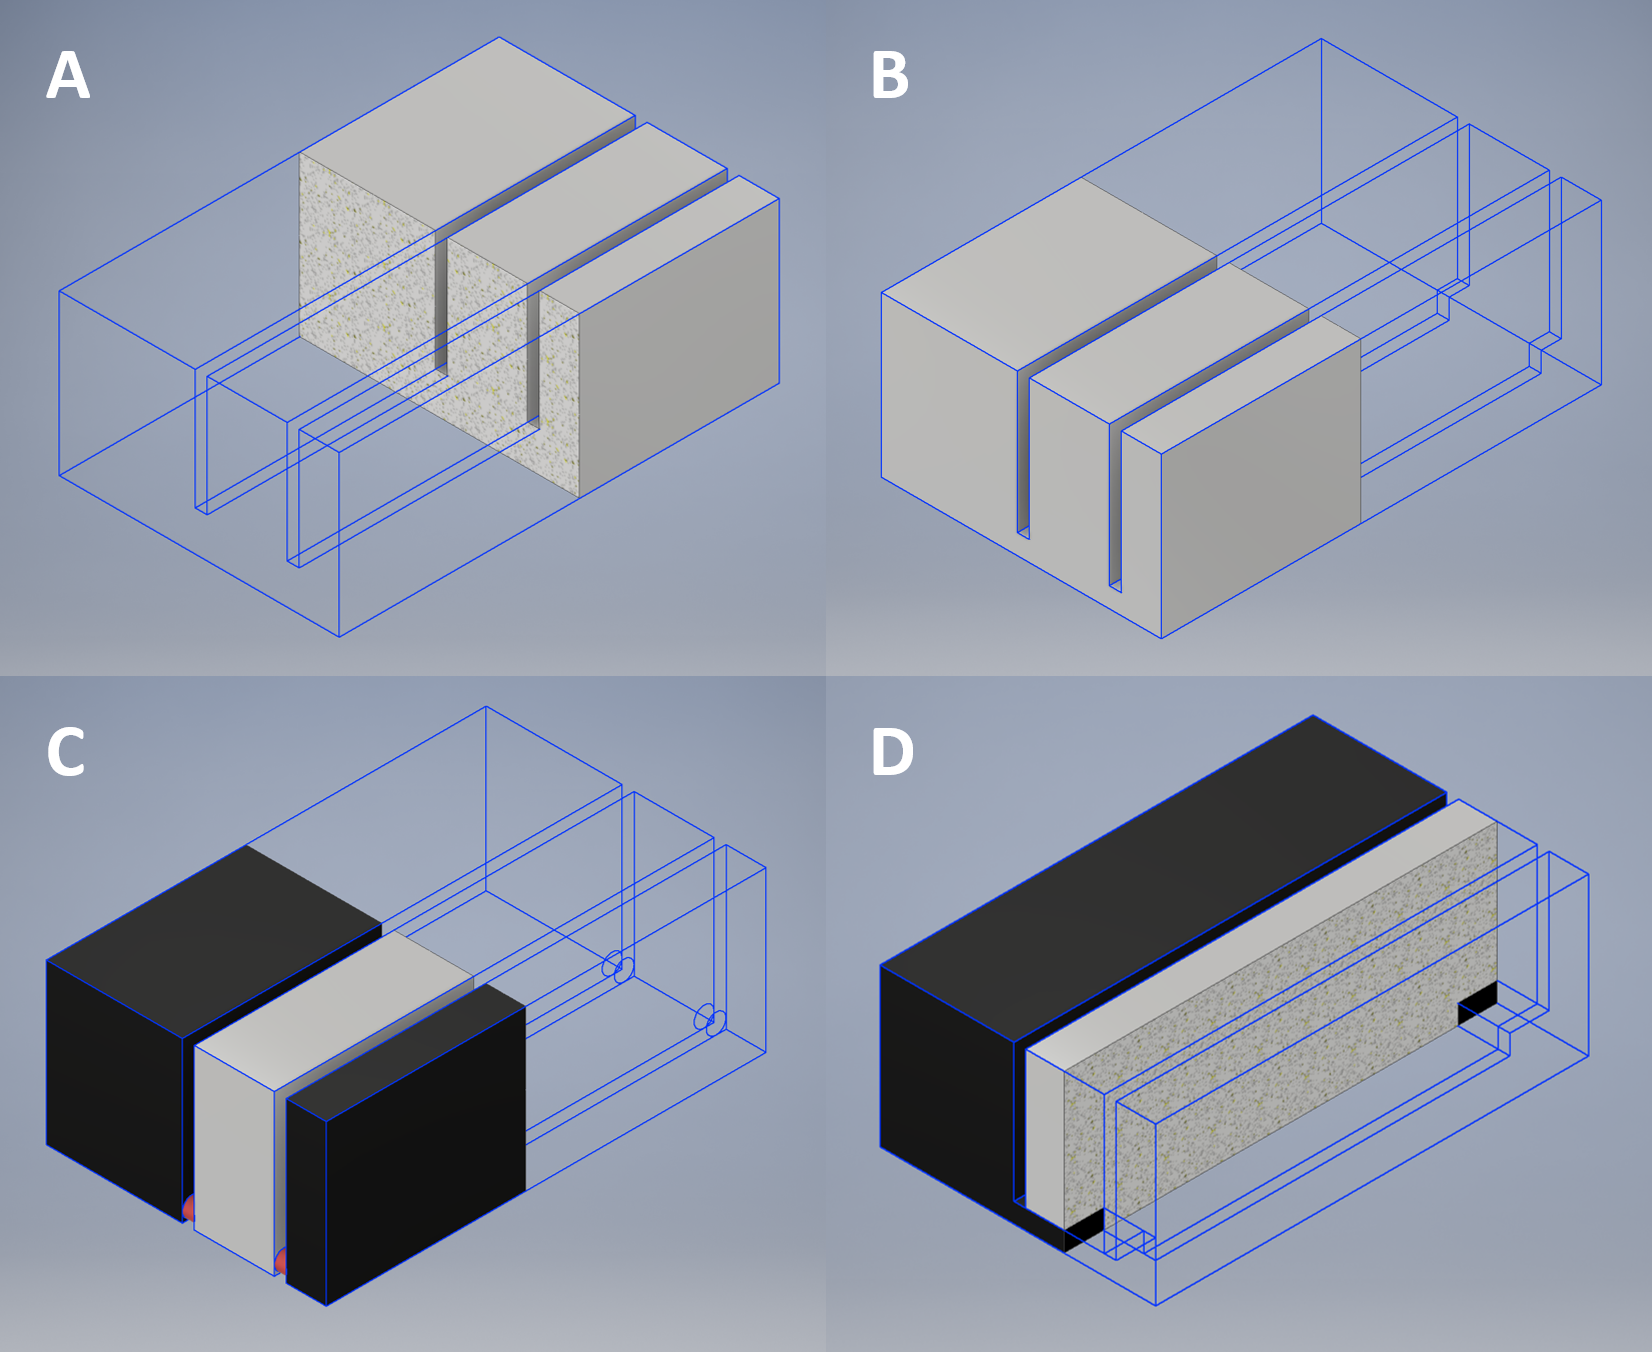
\includegraphics[width = \textwidth]{splitconcepts.png}
	\caption[Thermal Insulation Concepts.]{CAD representations of the thermal insulation concepts.}
	\label{fig:splitconcepts}
\end{figure}ˆ 
\FloatBarrier

Concept A features a groove machined into a solid billet of Aluminium, forming an air gap between the two regions. This concept has the advantage of simplicity, aiding with manufacture and serviceability. It's use of a single piece of material is also cost effective. It however had two main drawbacks. With the groove limited to a maximum of 3mm width and therefore 30mm deep, there is a large portion of material remaining which joins the two regions, leading to an undesirable level of heat transfer. Furthermore, the tooling costs involved with manufacturing this concept with the high aspect ration groove are significantly higher than with traditional machining operations. For these reasons, this concept required further development.\\

Concept B furthered the ideal behind Concept A by improving on some of its flaws, namely the transfer of heat. This was achieved by including further machining operations on the bottom face of the block. Therefore, the groove depth could be through the thickness of the block, apart from the small connecting regions on the outer edges of each groove. This simple change allowed the connecting area of material to be reduced to only 10\% of that of Concept A. Despite these improvements, the extra operations still require that small sections be machined at the same 30mm depth with the 3mm tool bit. Avoiding this is possible by performing machining operations on all four faces as opposed to only the top and bottom, however this will still carry added cost. Further to this, the homogeneous material and solid connection would allow for a more rapid heat transfer than was desirable. While aluminium is required for the Thermal Region due to its high level of heat transfer, this will result in large energy losses to the Carrier. It was therefore decided that the insulation should also make use of a thermally insulation material along with the physical separation used in the concepts to date.\\



\subsubsection{Heater Selection}

In order to achieve the heating requirements of the extraction process, two main heating devices were considered, as were explored in Chapter \ref{cha:literaturereview}, Literature Review. These were the solid state TEC and the resistive heat strip.

\subsection{Temperature Controller}

\subsection{Magnetic Separation}

\section{Magnetic Separation Station}

\subsection{Magnetic Separation}

\subsection{Waste Disposal}